\documentclass[fullscreen=true, bookmarks=true, hyperref={pdfencoding=unicode}]{beamer}
\usepackage[utf8]{inputenc}                                % Кодировка
\usepackage[english,russian]{babel}                        % Переносы
\usepackage{xcolor}                                        % Работа с цветом
\usepackage{amsmath,amssymb,amsfonts}                      % Символы АМО
\usepackage{graphicx}                                      % Графика
\usepackage[labelsep=period]{caption}                      % Разделитель в подписях к рисункам и таблицам
\usepackage{hhline}                                        % Для верстки линий в таблицах
\usepackage{tikz}                                          % Для простых рисунков в документе
\usepackage{fancybox}                                      % Пакет для отрисовки рамок
\usepackage{verbatim}                                      % Для вставки кода в презентацию
\usepackage{animate}                                       % Для вставки видео в презентацию
\usepackage{xmpmulti}                                      % Для вставки gif в презентацию
\usepackage{multirow}

\usetikzlibrary{arrows,snakes,backgrounds}                 % Для отрисовки стрелок

\graphicspath{{images/}}                                   % Путь до рисунков
\setbeamertemplate{caption}[numbered]                      % Включение нумерации рисунков

\definecolor{links}{HTML}{2A1B81}                          % blue for url links
\hypersetup{colorlinks,linkcolor=,urlcolor=links}          % nothing for others

\usetheme{Boadilla}
\usecolortheme{whale}

\usepackage{minted}

% \setbeameroption{show notes}
\setbeameroption{hide notes}
% \setbeameroption{show only notes}

\title{Lecture 7. Convolutional Neural Networks, advanced technics}
\author{Alex Avdyushenko}
\institute{Kazakh-British Technical University}
\date{October 24, 2022}
\titlegraphic{
\includegraphics[keepaspectratio,width=0.4\textwidth]{logo_kbtu.png}}

\begin{document}
%\unitlength=2mm

% выводим заглавие
\begin{frame}
\transdissolve[duration=0.2]
\titlepage
\end{frame}

\note{Hello, today we continue to talk about Convolutional Neural Networks, advanced optimization methods and architecture.

And again we will start with three questions for five minutes based on the materials of the previous lecture.}

\begin{frame}
  \frametitle{Five-minutes block}
  \pause
  \begin{itemize}
    \item Define a convolution operation for neural networks
    \item Write down the main features of the AlexNet network
    \item Write the formulas for updating the weights in the Momentum method
  \end{itemize}

\note{Please, write answers or send photos with them directly to me in private messages here in Teams, so that others cannot read your message. Last time, a lot of people did it, so I believe that this time you all will succeed.}

\end{frame}


{ % all template changes are local to this group.
    \setbeamertemplate{navigation symbols}{}
    \begin{frame}<article:0>[plain]
        \begin{tikzpicture}[remember picture,overlay]
            \node[at=(current page.center)] {
                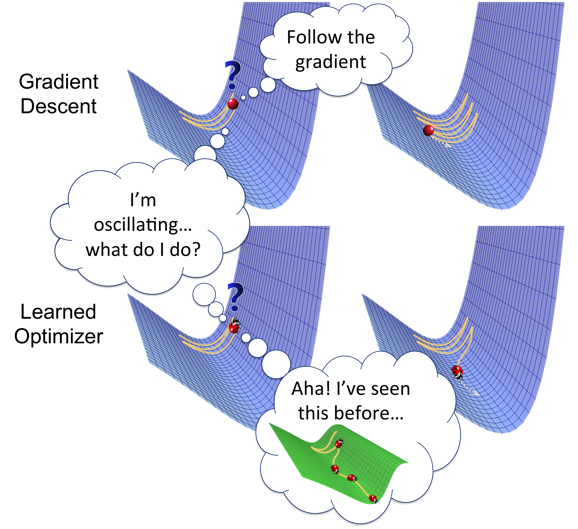
\includegraphics[keepaspectratio,
                                 width=\paperwidth,
                                 height=\paperheight]{optimization_mem.png}
            };
        \end{tikzpicture}
     \end{frame}
}

\note{Let's look at this picture. In many ways, it reflects the entire content of today's lecture.}

\begin{frame}
  \frametitle{Neural networks optimization methods}
  \framesubtitle{Recall the Momentum method}
  \pause
   \begin{columns}
     \begin{column}{0.45\paperwidth}
     Momentum accumulation method [B.T.Polyak, 1964] — exponential moving average of the gradient over $\frac{1}{1-\gamma}$ last iterations:

     $$\nu = {\color{red}\gamma} \nu + {\color{red}(1-\gamma)} \mathcal{L}_i^\prime(w)$$
     
     $$w = w - \eta \nu$$
     \end{column}
     \begin{column}{0.45\paperwidth}
     \centering
     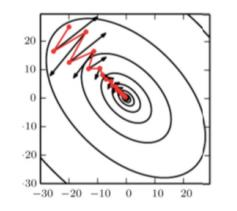
\includegraphics[keepaspectratio,
                      width=0.3\paperwidth]{momentum_2.jpg}
     \end{column}
   \end{columns}

   \note{A very popular method for improving the convergence of SGD is the momentum accumulation method. In it, from a physical point of view, the derivative of the loss function becomes the acceleration of the change in model parameters, and not the speed as in classical SGD.}
\end{frame}


\begin{frame}{AdaGrad}
  \pause
   \begin{align*}
      G &= G + \mathcal{L}_i^\prime(w) \odot \mathcal{L}_i^\prime(w) \\
      w &= w - {\eta_t} {\mathcal{L}_i^\prime(w)}\oslash{\sqrt{G + \varepsilon}}
   \end{align*}

   $\eta_t$ can be fixed, for example $\eta_t = 0.01$,

   $\odot, \oslash$ — component-wise multiplication and division of vectors

  \pause
   Advantages:
   \begin{itemize}
     \item $\mathcal{L}_i^\prime(w)$ — gradient on $i$-th object
     \item separate choice of adaptation for each direction
     \item is suitable for sparse data
   \end{itemize}

  \pause
  Disadvantage:
  \begin{itemize}
    \item $G$ is constantly increasing, which can cause learning to stop
  \end{itemize}

   \note{Another interesting approach is the adaptive gradient method. You accumulate squares of gradient vector and then change the model parameters by the component-wise way.}

\end{frame}


\begin{frame}
  \frametitle{RMSProp (running mean square)}

  \pause
   Equalization of rates of change of weights by moving average
   \begin{align*}
      G &= {\color{red}\alpha} G + {\color{red}(1 - \alpha)}\mathcal{L}_i^\prime(w) \odot \mathcal{L}_i^\prime (w) \\
      w &= w - {\eta_t} {\mathcal{L}_i^\prime(w)}\oslash{\sqrt{G + \varepsilon}}
   \end{align*}

   $\eta_t$ can be fixed, for example $\eta_t = 0.01$

  \pause
   Advantages:
   \begin{itemize}
     \item same as AdaGrad
     \item and $G$ does not grow uncontrollably
   \end{itemize}

  \pause
  Disadvantages:
  \begin{itemize}
    \item at the very beginning of training $G$ is averaged over zero previous values
    \item no moment count
  \end{itemize}

  \note{The development of AdaGrad is RMSProp — optimization method, which you really have in modern libraries.}

\end{frame}


\begin{frame}[t]
  \frametitle{Adam (adaptive momentum)}

  \pause
  \begin{align*}
  \nu &= \gamma \nu + (1-\gamma) \mathcal{L}_i^\prime(w) \quad     &\hat\nu = \nu(1-\gamma^k)^{-1} \\
    G &= {\alpha} G + {(1 - \alpha)}\mathcal{L}_i^\prime(w) \odot \mathcal{L}_i^\prime(w) \quad &\hat G = G(1-\alpha^k)^{-1} \\
    w &= w - {\eta_t}\hat\nu \oslash (\sqrt{\hat G + \varepsilon})
  \end{align*}

  $k$ — iteration number, $\gamma = 0.9, \alpha = 0.999, \varepsilon = 10^{-8}$

  \pause
  Advantages:
    \begin{itemize}
      \item are almost the same as RMSProp
      \item calibration $\hat\nu, \hat G$ increases $\nu, G$ on the first iterations
      \item is count of moment
    \end{itemize}

  \note{Adam is also one of modern optimization method, which you really may meet in modern applications.}

\end{frame}


\begin{frame}[t]
  \frametitle{Nadam (Nesterov-accelerated adaptive momentum)}

Same formulas for $\nu, \hat\nu, G, \hat G$

   $ w = w - {\eta_t}\left({\color{red}\gamma}\hat\nu + {\color{red}\frac{1-\gamma}{1-\gamma^k}\mathcal{L}_i^\prime (w)} \right) \oslash (\sqrt{\hat G+\varepsilon})$

   $k$ — iteration number, $\gamma = 0.9, \alpha = 0.999, \varepsilon = 10^{-8}$

   \noindent\rule{8cm}{0.4pt}

   {\it T. Dozat}. Incorporating Nesterov Momentum into Adam. ICLR-2016.

  \note{And Nadam (Nesterov-accelerated adaptive momentum) — is modern modification of Adam method.}
\end{frame}


\begin{frame}
  \frametitle{Convergence example}
  \begin{center}
    \animategraphics[loop,width=0.5\paperwidth,autoplay]{8}{gd_animation-}{0}{118}
  \end{center}

  \noindent\rule{8cm}{0.4pt}

   {\small Source: \href{http://www.denizyuret.com/2015/03/alec-radfords-animations-for.html}{http://www.denizyuret.com/2015/03/alec-radfords-animations-for.html}}

  \note{Let's look on example of convergence of considered optimization methods.}
\end{frame}


\begin{frame}
    \begin{block}{Question}
    Which method and how to choose?
    \end{block}
\end{frame}


\begin{frame}
  \frametitle{Gradient exploding}
  \begin{center}
    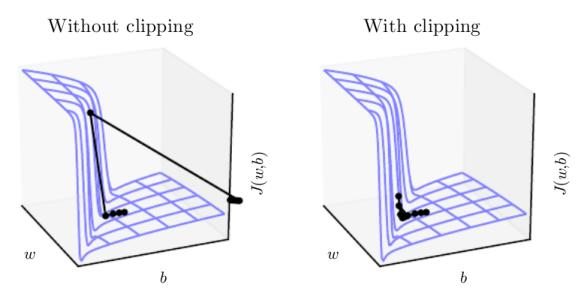
\includegraphics[keepaspectratio,
                     width=0.6\paperwidth]{gradient_exploding.jpg}
  \end{center}
  
  You need to numpy.clip by value or by absolute value.

  \noindent\rule{8cm}{0.4pt}

  {\small Source: \href{https://neptune.ai/blog/understanding-gradient-clipping-and-how-it-can-fix-exploding-gradients-problem}{https://neptune.ai/blog/understanding-gradient-clipping-and-how-it-can-fix-exploding-gradients-problem}}

  \note{There is typical problem in neural network optimization, it is gradient exploding.}
\end{frame}


\begin{frame}
\frametitle{Regularization Methods}

   \pause
   {\bf Dropout} is a method of random shutdowns of neurons

   \pause
   {\bf Learning stage}: make the gradient step $\mathcal{L}_i(w) \to \min\limits_w$, disable the $h$-th neuron of the $\ell$-th layer with probability $p_\ell$:

   $x_{ih}^{\ell + 1} = {\color{red}\xi_h^\ell} \sigma_h (\sum\limits_j w_{jh} x_{ij}^\ell), \ \ \
    {\color{red}P(\xi_h^\ell = 0) = p_\ell}$

   \pause
   {\bf Application stage}: turn on all neurons, but with a correction:

   $x_{ih}^{\ell + 1} = {\color{red}(1 - p_\ell)} \sigma_h(\sum\limits_j w_{jh} x_{ij}^\ell)$

   \pause
   \begin{center}
     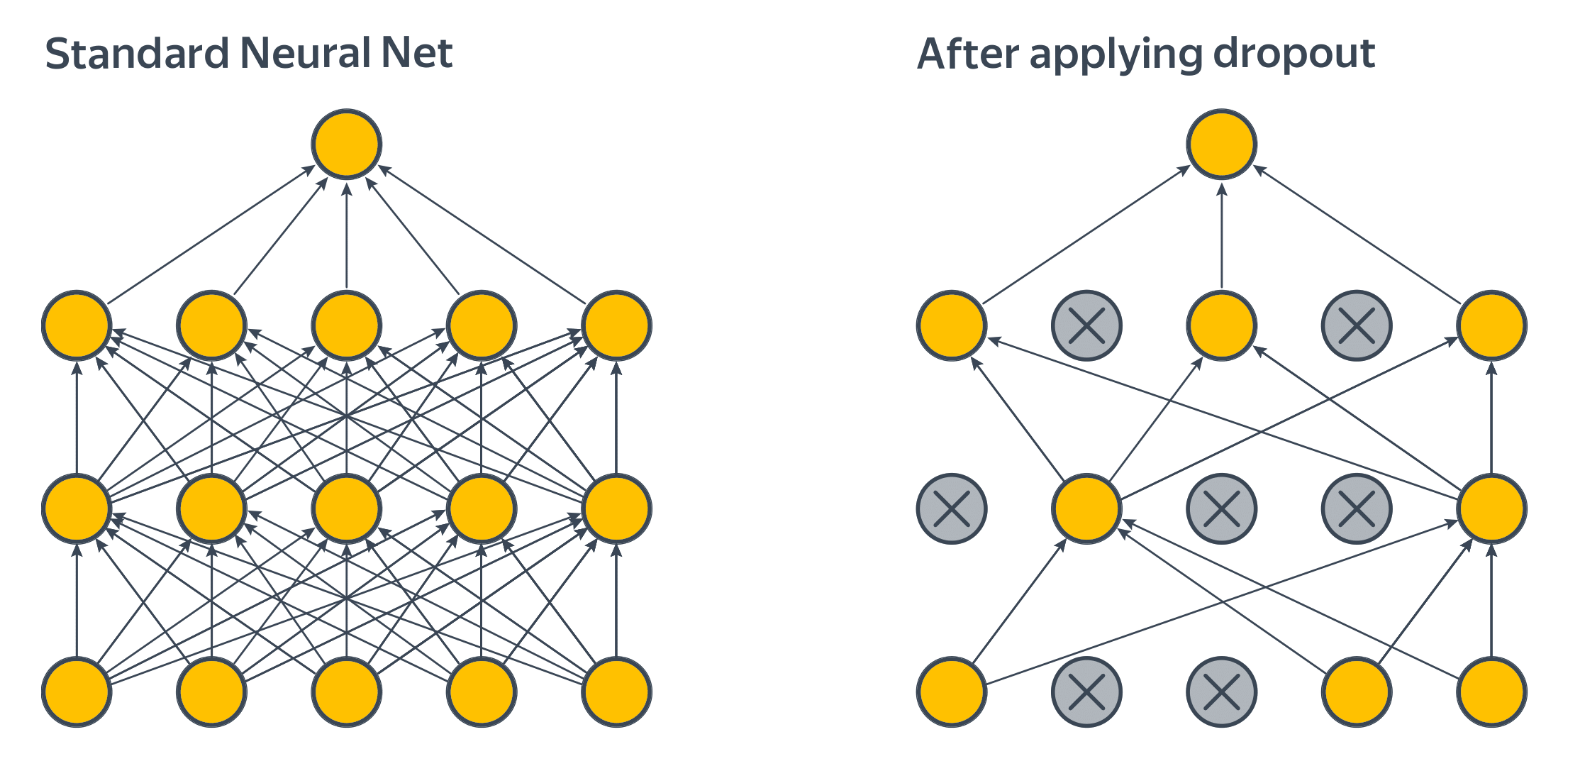
\includegraphics[keepaspectratio,
                      width=.6\paperwidth]{dropout_shad.png}
   \end{center}

   \note{Dropout is a method of random shutdowns of neurons. It has two stages: learning stage and application stage.}

\end{frame}


\begin{frame}
    \begin{block}{Question}
    What is the peculiarity of this case of dropout implementation?
    \end{block}
\end{frame}


\begin{frame}
\frametitle{Inverted Dropout}
    In practice {\bf Inverted Dropout} is used

    \pause
    {\bf Learning stage}:
   $$x_{ih}^{\ell + 1} = {\color{red}\frac{1}{1-p_\ell} \xi_h^\ell} \sigma_h (\sum\limits_j w_{jh} x_{ ij}^\ell), \ \ \
    P(\xi_h^\ell = 0) = p_\ell$$

    \pause
   {\bf Application stage} doesn't require neither modification nor knowledge of $p_\ell$:
   $$x_{ih}^{\ell + 1} = \sigma_h(\sum\limits_j w_{jh} x_{ij}^\ell)$$

   $L_2$-regularization prevents growth of training parameters:
   $$\mathcal{L}_i(w) + \frac{\lambda}{2} \|w\|^2 \to \min\limits_w$$

   Gradient step with Dropout and $L_2$ regularization:
   $$w = w (1 - \eta \lambda) - \eta{\color{red}\frac{1}{1-p_\ell} \xi_h^\ell} \mathcal{L}_i^\prime(w )$$
\end{frame}


\begin{frame}
  \frametitle{Dropout interpretations}

  \begin{itemize}
    \pause
    \item we approximate simple voting over $2^N$ networks with a common set of $N$ neurons
    \pause
    \item regularization: we choose from all networks the most resistant to the loss of $pN$ neurons, simulating the reliability of the brain
    \pause
    \item reducing retraining by forcing different parts of the network to solve the same original task
  \end{itemize}
  \pause
  \begin{center}
    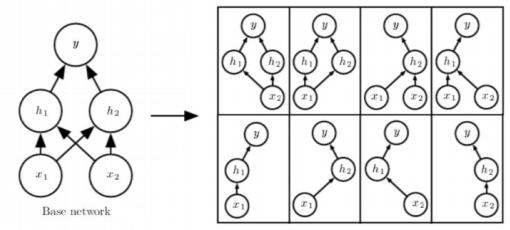
\includegraphics[keepaspectratio,
                     width=0.5\paperwidth]{dropout_interpretation.jpg}
  \end{center}
\end{frame}


\begin{frame}
  \frametitle{Batch normalization}

  $B = \{ x_i\}$ — mini-batch of whole dataset

  Averaging the $\mathcal{L}_i(w)$ gradients over the batch speeds up the convergence.

   $B^\ell = \{ u_i^\ell\}$ — vectors of $x_i$ objects at the output of the $\ell$-th layer

  \pause
   1. Normalize each $j$-th component of the vector $u_i^\ell$ by the batch

  $$
    \hat u_{ij}^\ell = \frac{u_{ij}^\ell - \mu_j}{\sqrt{\sigma_j^2 + \varepsilon}}; \quad
    \mu_j = \frac{1}{|B|} \sum\limits_{x_i \in B} u_{ij}^\ell; \quad
    \sigma_j^2 = \frac{1}{|B|} \sum\limits_{x_i \in B} (u_{ij}^\ell - \mu_j)^2
  $$

  \pause
  2. Add a linear layer with custom weights:

   $$ \tilde u_{ij}^\ell = \gamma_j^\ell \hat u_{ij}^\ell + \beta_j^\ell $$

  \pause
  3. Parameters $\gamma_j^\ell, \beta_j^\ell$ are configured by BackProp

  \note{Let's go on to the next important regulzrization method. It is Batch normalization method.}

\end{frame}


\begin{frame}
  \frametitle{Initial Approximation of the Weights}
  \begin{center}
    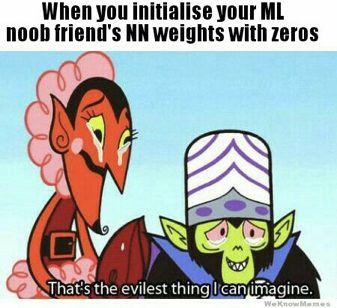
\includegraphics[keepaspectratio,
                     width=.4\paperwidth]{weight_init_meme.jpg}
  \end{center}

  \note{Also of course very important to choose consistently the Initial Approximation of the Weights.}

\end{frame}


\begin{frame}
  \frametitle{Monitoring changes in variances}
     \framesubtitle{Both of neuron values and backpropagation gradients}
   
   Equalization of variances of both neurons and gradients in different layers — Xavier initialization for $\tanh$:

   $$ w_j \sim U \left[ -\frac{{6}}{\sqrt{n_{in}+n_{out}}}, \frac{{6}}{\sqrt{n_{in}+n_ {out}}} \right]$$

   $n_{in},\ n_{out}$ — the number of neurons in the previous and current layers, respectively

   The proof and details are \href{https://ml-handbook.ru/chapters/neural_nets/training}{in the SHAD textbook (in Russian yet)}.
   \pause
   \begin{block}{Question}
   What to do in case of ReLU activation?
   \end{block}

  \note{In fact, the consistently rule is quite simple — you need to make sure that the variance of the layers is preserved both during the forward and backward pass through the neural network.}
\end{frame}


\begin{frame}
  \frametitle{Other ways of initialization}
   \begin{enumerate}
     \item Layer-by-layer training of neurons as linear models
       \begin{itemize}
         \item or by random subsample
         \item or by a random subset of inputs
         \item or from various random initial distributions
       \end{itemize}

     This ensures the diversity of neurons.

     \item Weight initialization of a pre-trained model (for example, an autoencoder)
   \end{enumerate}
\end{frame}


\begin{frame}
\frametitle{ResNet — Residual Net}

   Skip-connection of the $\ell$ layer with the previous $\ell - d$ layer:

   $$ x_\ell = \sigma(Wx_{\ell-1}) + x_{\ell-d}$$

   The $\ell$ layer learns not the new vector representation $x_\ell$, but its increment $x_\ell - x_{\ell-d}$

   \begin{center}
     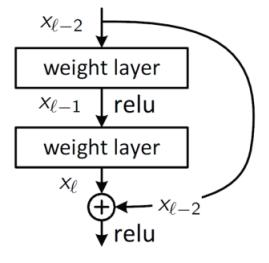
\includegraphics[keepaspectratio,
                      width=.3\paperwidth]{skip-connection.jpg}
   \end{center}

  \note{Great, now let's talk a bit about modern neural network architectures.}

\end{frame}


\begin{frame}
  \begin{itemize}
     \item (main) it is possible to increase the number of layers
     \item increments are more stable $\to$ convergence is better
   \end{itemize}

  \vspace{1cm}
  \noindent\rule{8cm}{0.4pt}

  {\it Kaiming He, Xiangyu Zhang, Shaoqing Ren, Jian Sun.} Deep Residual Learning for Image Recognition. 2015.

  {\it R.K. Srivastava, K. Greff, J. Schmidhuber.} Highway Networks. 2015
\end{frame}


\begin{frame}
  \frametitle{ResNet: visualization of loss function}

\begin{center}
  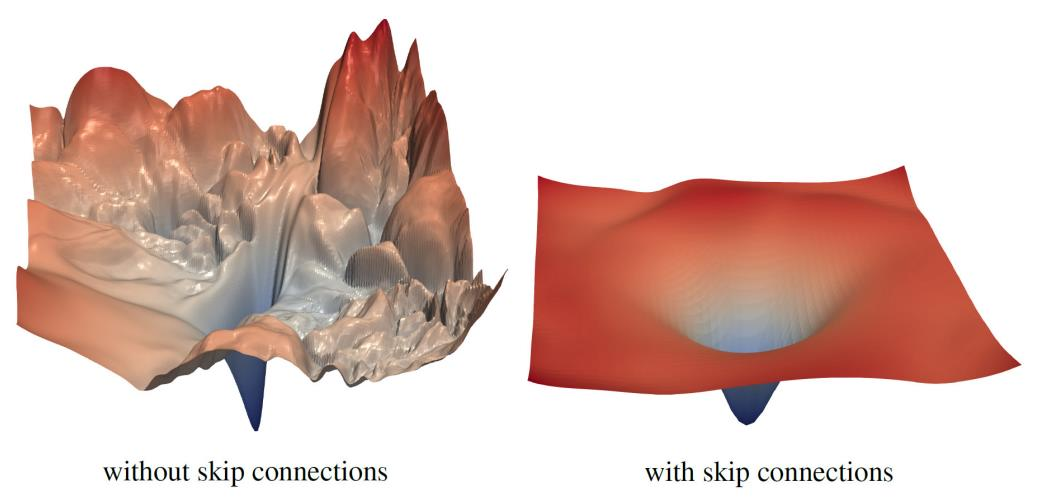
\includegraphics[keepaspectratio,
                   width=0.7\paperwidth]{skip-connection-opt.jpg}
\end{center}

  \noindent\rule{8cm}{0.4pt}

  {\it Hao Li et al.} Visualizing the Loss Landscape of Neural Nets. 2018.

  \note{This is famous image from a paper that almost became a meme in deep learning :)}
\end{frame}


\begin{frame}
  \frametitle{WideResNet — WRN}
  Disadvantages of ResNet
  \begin{itemize}
    \item is too deep — up to 1000 layers :)
    \item take a long time to train to SotA
  \end{itemize}
  \begin{center}
    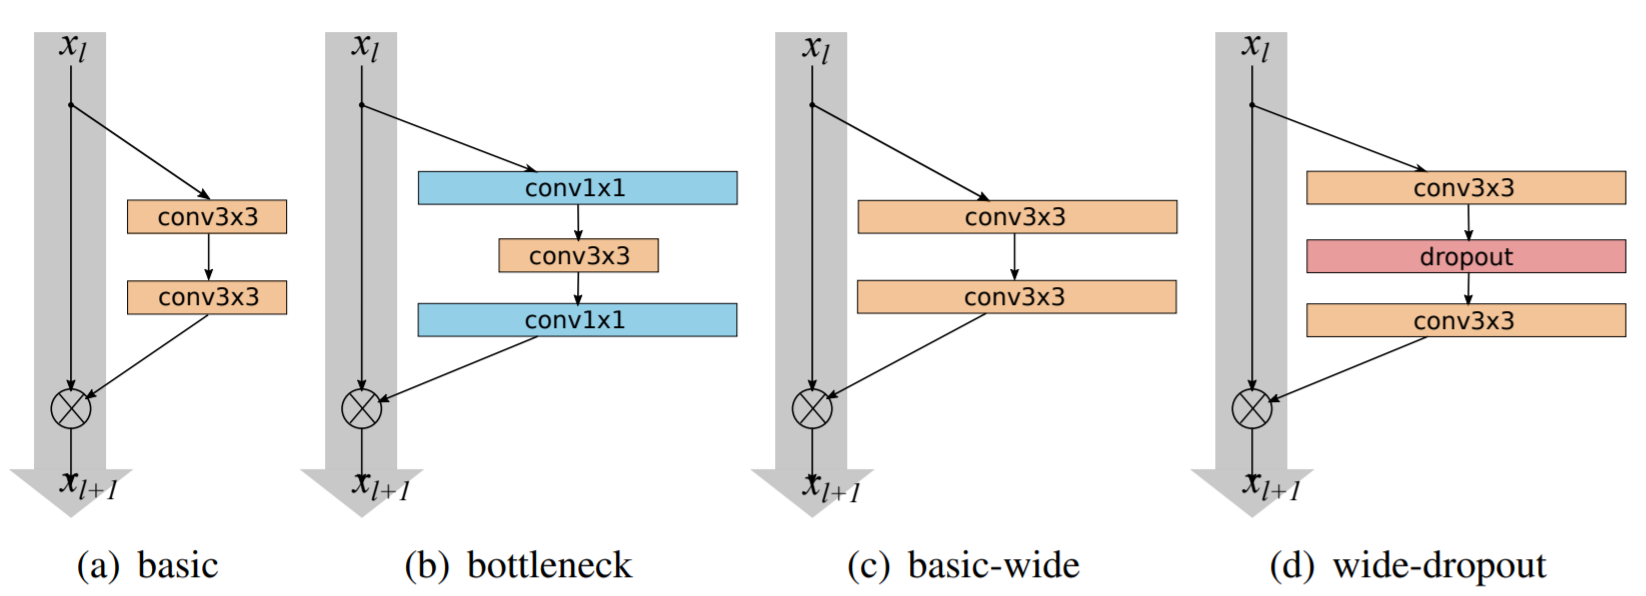
\includegraphics[keepaspectratio,
                     width=0.6\paperwidth]{wrn_blocks.png}
  \end{center}

  \begin{itemize}
    \item a simple WRN network of 16 layers defeated all ResNets
    \item WRN-40-4 (i.e. 40 layers and 4x width) trains 8 times faster than ResNet-1001
  \end{itemize}

  \noindent\rule{8cm}{0.4pt}

  {\it S. Zagoruyko, N. Komodakis} \href{https://arxiv.org/pdf/1605.07146.pdf}{Wide Residual Networks, 2017}

  \note{And the final architecture for today's lecture WideResNet, which I recommend paying attention to when solving the competition from the second homework. It has already been posted on github and in teams.}

\end{frame}


\begin{frame}
  \frametitle{Summary}
   \begin{itemize}
     \item Convolutional networks are very well suited for image processing
     \item Various optimization algorithms: adam, RMSProp
     \item Regularization methods: dropout, $L_2$ and batch normalization
     \item The choice of the initial approximation is also important (weight initialization)
     \item ResNet and skip-connections, WideResNet
   \end{itemize}

   \pause
   What else can you see?
   \begin{itemize}
     \item Course lecture at Stanford \href{https://www.youtube.com/watch?v=DAOcjicFr1Y}{about convolutional networks}
   \end{itemize}
\end{frame}


\begin{frame}
  \frametitle{Levenberg-Marquardt Diagonal Method}
  \framesubtitle{Reminder}
  Newton-Raphson method (second order):

  $$ w = w - \eta(\mathcal{L}^{\prime\prime}_i(w))^{-1} \mathcal{L}^{\prime}_i(w),$$

  where $\mathcal{L}^{\prime\prime}_i(w) = 
  \frac{
  \partial^2 \mathcal{L}_i(w)}
  {\partial w_{jh} \partial w_{j^\prime h^\prime}}$ — Hessian

  {\bf Heuristics}. We assume that the Hessian is diagonal:

    $w_{jh} = w_{jh} - \eta \left(\frac{\partial^2 \mathcal{L}_i(w)}{\partial w^2_{jh}} + \mu \right)^{-1} \frac{\partial \mathcal{L}_i(w)}{\partial w_{jh}}$,

    $\eta$ is the learning rate, we can assume $\eta = 1$

    $\mu$ — a parameter that prevents the denominator from being set to zero

    The ratio $\eta/\mu$ is the learning rate on flat sections of the functional $\mathcal{L}_i(w)$, where the second derivative vanishes.
\end{frame}

\end{document}
